\documentclass{subfiles}[../main.tex]

\begin{document}
    \section{Semaine 2} % (fold)
    \label{sec:Semaine 2}
        \subsection{Mardi le 9 Mai} % (fold)
        \label{sub:Mardi le 9 Mai}

            % Journée du mardi le 9 mai
            \subsubsection{Changement de base} % (fold)
            \label{sec:Changement de base}
            Soit effectuons le changement de base de l'Hamiltonien de Hubbard.
            \begin{align}
                H=U\sum_{i}n_{i\uparrow}n_{i\downarrow}
                -\sum_{<i,j>,\sigma}t_{ij}\qty(
                    c^\dagger_{i,\sigma}c_{j,\sigma}
                    +
                    c^\dagger_{j,\sigma}c_{i,\sigma}
                )
            \end{align}
            Les transformées de Fourrier des opérateurs création et
            annihilation sont
            \begin{align}
                c^\dagger_{i,\bm{k}}&=\frac{1}{\sqrt{N}}\sum_{\bm{r}}
                e^{i\bm{k}\cdot\bm{r}}
                c^\dagger_{i,\bm{r}}\\
                c^\dagger_{i,\bm{r}}&=\frac{1}{\sqrt{N}}\sum_{\bm{k}}
                e^{-i\bm{k}\cdot\bm{r}}
                c^\dagger_{i,\bm{r}}
            \end{align}
            Allons-y terme à terme.

            % subsubsection Changement de base (end)
            \subsubsection{Hubbard Intro Old} % (fold)
            \label{sec:Hubbard Intro Old}
            % Problème 1:
            \begin{problem}
                Supposons que $N=2$.
            Construire une représentation matricielle
            explicite, dans l'espace de Hilbert global
            de dimension $2^2=4$, des opérateurs suivants:
            $c_1,c_2,n_1,n_2$
            \end{problem}
            Soit la base de l'espace de Hilbert
            \begin{align}
                \left\{
                \ket{00},\ket{01},\ket{10},\ket{11}
                    \right\}
            \end{align}
            On sait que $c_1$ détruit le premier site, tandis que $c_2$ détruit
            le second, on peut donc les écrires en terme de mapping entre les
            états
            \begin{align}
                c_1:\quad\left\{
                    \ket{00}\rightarrow\bm{0},
                    \ket{01}\rightarrow\ket{00},
                    \ket{10}\rightarrow\bm{0},
                    \ket{11}\rightarrow\ket{10}
                    \right\}\\
                c_2:\quad\left\{
                    \ket{00}\rightarrow\bm{0},
                    \ket{01}\rightarrow\bm{0},
                    \ket{10}\rightarrow\ket{00},
                    \ket{11}\rightarrow\ket{01}
                    \right\}
            \end{align}
            Et donc si on écrit les états suivants
            \begin{align}
                \ket{00}&=\begin{pmatrix}
                    1\\0\\0\\0
                \end{pmatrix}\\
                \ket{01}&=\begin{pmatrix}
                    0\\1\\0\\0
                \end{pmatrix}\\
                \ket{10}&=\begin{pmatrix}
                    0\\0\\1\\0
                \end{pmatrix}\\
                \ket{11}&=\begin{pmatrix}
                    0\\0\\0\\1
                \end{pmatrix}
            \end{align}
            On obtient les matrices
            \begin{align}
                c_1&=\begin{pmatrix}
                    0&1&0&0\\
                    0&0&0&0\\
                    0&0&0&1\\
                    0&0&0&0
                \end{pmatrix}\\
                c_2&=\begin{pmatrix}
                    0&0&1&0\\
                    0&0&0&1\\
                    0&0&0&0\\
                    0&0&0&0
                \end{pmatrix}
            \end{align}

            % Problème 2:
            \begin{problem}
                Supposons que $N=2$ et
            considérons un état général à un électron
            $\ket{\psi}=\alpha\ket{1}+\beta\ket{2}$,
            où $\abs{\alpha}^2+\abs{\beta}^2=1$. Quelle
            est la probabilité que l'électron soit sur
            l'ion no $1$? Quelles sont les valeurs moyennes
            de $n_1$ et $n_2$?
            \end{problem}
            La probabilité d'être sur le site $1$ est
            \begin{align}
                \abs{\braket{1}{\psi}}^2&=\abs{\alpha}^2
            \end{align}
            Les valeurs moyennes sont
            \begin{align}
                \ket{1}=\ket{01}\quad&\quad\ket{2}=\ket{10}\\
                \bra{\psi}n_1\ket{\psi}&=\abs{\alpha}^2\\
                \bra{\psi}n_2\ket{\psi}&=\abs{\beta}^2
            \end{align}

            % Problème 3:
            \begin{problem}
                Considérer un modèle
            à $N=4$ sites et comportant $M=4$ électrons,
            avec $t=0$. Trouver les deux niveaux d'énergie
            les plus bas avec les états correspondants.
            Combien y en a-t-il pour chacun des deux
            niveaux?
            \end{problem}
            Pour $t-0$, le Hamiltonien de Hubbard devient
            \begin{align}
                H=V&=U\sum_{i}n_{i\uparrow}n_{i\downarrow}
            \end{align}
            Avec $M=3$ électrons, le fondamental est celui que les trois
            électrons sont sur des sites différents, dégénérés plusieurs fois
            avec une énergie de $E=0$. Le premier état excité est celui qui
            a un site avec deux électrons de spins opposés, avec une énergie de
            $E=U$, $4$ fois dégénéré.

            % Problème 4:
            \begin{problem}
                Démontrer la relation 22
            et ensuite que les deux équations de 20 sont
            compatibles.
            \end{problem}
            Commençons par $r=0$, soit
            \begin{align}
                \sum_{k}e^{ikr}=\sum_k 1=N
            \end{align}
            Ensuite, allons-y avec $r\neq 0$.
            \begin{align}
                \sum_{j=0}^{N-1}e^{ir(2\pi j/N)}&=\frac{1-e^{2\pi ir}}
                {1-e^{2\pi ir/N}}
            \end{align}
            Comme $r$ est un point du réseau, alors il s'agit d'un entier. Le
            numérateur s'annule donc, ce qu'il fallait démontrer.

            % Problème 5:
            \begin{problem}
                Démontrer que les opérateurs
                $\widetilde{c_\sigma}(\bm{k})$ et
                $\widetilde{c_\sigma}(\bm{k})$ satisfont
                aux relations d'anticommutation suivantes:
                \begin{align}
                    &\{\widetilde{c}_\sigma(\bm{k}),
                    \widetilde{c}_{\sigma'}(\bm{k'})\}=0
                    &&\{\widetilde{c}_\sigma(\bm{k}),
                    \widetilde{c}_{\sigma'}^\dagger(\bm{k'}
                    )\}=\delta_{\sigma\sigma'}
                    \delta_{\bm{k}\bm{k'}}
                \end{align}
            \end{problem}
            Partons des relations d'anti-commutation des opérateurs définis
            précédemment
            \begin{align}
                &\{c_{i\sigma},c_{j,\sigma'}\}=0
                &&\{c^\dagger_{i\sigma},c^\dagger_{j,\sigma'}\}=0
                &&\{c_{i\sigma},c^\dagger_{j,\sigma'}\}=\delta_{ij}
                \delta_{\sigma\sigma'}
            \end{align}
            Soit alors les transformations de Fourier
            \begin{align}
                &\widetilde{c}_{\sigma}(k)=\frac{1}{\sqrt{N}}\sum_re^{-ikr}
                c_{\sigma}(r)
                &\widetilde{c}^\dagger_{\sigma}(k)=\frac{1}{\sqrt{N}}\sum_re^{ikr}
                c^\dagger_{\sigma}(r)
            \end{align}
            Alors, comme l'anti-commutateur est bilinéaire, on a que
            \begin{align}
                \{\widetilde{c}_\sigma(\bm{k}),
                    \widetilde{c}_{\sigma'}(\bm{k'})\}
                    =\frac1N\sum_{r,r'}e^{-irk-ir'k'}\{c_{\sigma}(r),
                    c_{\sigma'}(r')\}=0\\
                \{\widetilde{c}^\dagger_\sigma(\bm{k}),
                    \widetilde{c}^\dagger_{\sigma'}(\bm{k'})\}
                    =\frac1N\sum_{r,r'}e^{irk+ir'k'}\{c^\dagger_{\sigma}(r),
                    c^\dagger_{\sigma'}(r')\}=0\\
                \{\widetilde{c}_\sigma(\bm{k}),
                    \widetilde{c}^\dagger_{\sigma'}(\bm{k'})\}
                    =\frac1N\sum_{r,r'}e^{-irk+ir'k'}\{c_{\sigma}(r),
                    c^\dagger_{\sigma'}(r')\}=\frac1N\sum_re^{-ir(k-k')}
                    \delta_{\sigma\sigma'}\\
                    =\delta_{kk'}\delta_{\sigma\sigma'}
            \end{align}

            %Problème 6:
            \begin{problem}
                Démontrer que l'opérateur $K$ s'exprime
                comme suit en fonction des opérateurs
                $\widetilde{c_\sigma}(\bm{k})$ et
                $\widetilde{c_\sigma}^\dagger(\bm{k})$:
                \begin{align}
                    &K=-2t\sum_{\bm{k}\sigma}
                    \cos(k)n_\sigma(\bm{k})
                    &&n_\sigma(\bm{k})\equiv
                    \widetilde{c}_\sigma^\dagger(\bm{k})
                    \widetilde{c}_\sigma(\bm{k})
                \end{align}
            \end{problem}
            Soit l'opérateur $K$
            \begin{align}
                K&=-t\sum_{<i,j>,\sigma}\qty(c^\dagger_{i,\sigma}c_{j,\sigma}
                +c^\dagger_{j,\sigma}c_{i,\sigma})\\
                &=-t\sum_{R,r,\sigma}\qty(c^\dagger_{\sigma}(R+r)c_{\sigma}(R-r)
                +c^\dagger_{\sigma}(R-r)c_{\sigma}(R+r))
            \end{align}
            avec
            \begin{align}
                &R=\frac{r_1+r_2}{2}
                &&r=\frac{r_1-r_2}{2}
            \end{align}
            Alors
            \begin{align}
                K&=-\frac{t}{N}\sum_{R,r,\sigma,k,k'}\qty(
                    c^\dagger_{\sigma}(k)c_\sigma(k')e^{i(R+r)k-i(R-r)k'}+
                    c^\dagger_{\sigma}(k')c_\sigma(k)e^{i(R-r)k-i(R+r)k'}
                )\\
                &=-\frac{t}{N}\sum_{R,r,\sigma,k,k'}\qty(
                    c^\dagger_{\sigma}(k)c_\sigma(k')e^{ir(k+k')+iR(k-k')}+
                    c^\dagger_{\sigma}(k')c_\sigma(k)e^{-ir(k+k')+iR(k-k')}
                )\\
                &=-t\sum_{r,\sigma,k}\qty(
                    c^\dagger_{\sigma}(k)c_\sigma(k)e^{i2rk}+
                    c^\dagger_{\sigma}(k)c_\sigma(k)e^{-2irk}
                )\\
                &=-2t\sum_{r,\sigma,k}
                    c^\dagger_{\sigma}(k)c_\sigma(k)\cos(2kr)
            \end{align}

            %Problème 7:
            \begin{problem}
                Démontrer que les opérateurs de nombre
                $n_\sigma(\bm{k})$ associés à des spins ou
                des nombres d'ondes différents commutent.
            \end{problem}
            Les opérateurs création et annihilation associés à des nombres
            quantiques différents
            anticommutent. Alors, comme l'opérateur
            nombre est composé de deux opérateurs création et annihilation,
            il faut utiliser deux fois les relations d'anti-commutation pour
            faire traverser un autre opérateur création annihilation. Par
            conséquent, les opérateurs nombres et les opérateurs création
            annihilation associés à des nombres quantiques différents commutent.
            Il en va de soi que les opérateurs nombre associés à des nombres
            quantiques différents commutent.

            %Problème 8:
            \begin{problem}
                Quel est l'état fondamental d'un système de
                $N$ électrons installés sur un anneau de
                $N$ sites? On est à demi-remplissage, car
                la moitié du nombre maximum d'électrons ($2N$) sont présents.
            \end{problem}
            À demi-remplissage, l'état feromagnétique est l'état fondamental,
            comme c'est ainsi que l'on minimise le terme d'interaction, en
            limitant les paires d'électrons sur le même site. De plus, cette
            configuration minimise le terme de saut, car les électrons ne
            peuvent pas sauter aux sites voisins. On connait déjà le
            fondamental du terme $K$ à demi-remplissage, soit
            \begin{align}
                \widetilde{c}^\dagger_{\sigma_1}(k_1)(\cdots)
                \widetilde{c}^\dagger_{\sigma_N}(k_N)\ket{0}
            \end{align}
            un état propre de $K$. Sachant qu'il y a $N$ valeurs possibles de
            $k$ dans la première zone de Brillouin, alors l'énergie, pourvue

            %Problème 9:
            \begin{problem}
                Quelle est la probabilité de trouver deux électrons sur un même
                site dans l'état fondamental trouvé ci-dessus?
            \end{problem}

            % subsubsection Hubbard Intro Old (end)


        % subsection Mardi le 9 Mai (end)

        \subsection{Mercredi le 10 Mai}
            Deux problèmes à faire pour cette semaine, soit il faut montrer
            l'orthonormalité de l'ordre normal, et écrire un code qui diagonalise
            par bloc l'hamiltonien. Commençons par montrer que l'ordre normal
            est orthonormé.
            \subsubsection{Orthonormalité de l'ordre normal.} % (fold)
            \label{sec:orthonormalité de l'ordre normal.}
                Soit l'ordre normal
                \begin{align}
                    c^\dagger_{1\uparrow}c^\dagger_{2\uparrow}(\cdots)
                    c^\dagger_{1\downarrow}c^\dagger_{2\downarrow}(\cdots)
                    \ket{\{0\}^N}
                \end{align}

            % subsubsection orthonormalité de l'ordre normal. (end)

        \subsection{Jeudi le 11 Mai} % (fold)
        \label{sub:Jeudi le 11 Mai}
            Le but est de faire rouler le code de Peter. Voici la figure obtenue
            en roulant le \texttt{tutorial\_updated}. Quelques problèmes ont été
            rencontrés, notes que j'ai compilées dans le fichier
            \texttt{patches.md}. En changeant les paramètres, je ne suis pas
            capable de reproduire les autres figures.
            \begin{figure}[h!]
                \begin{center}
                    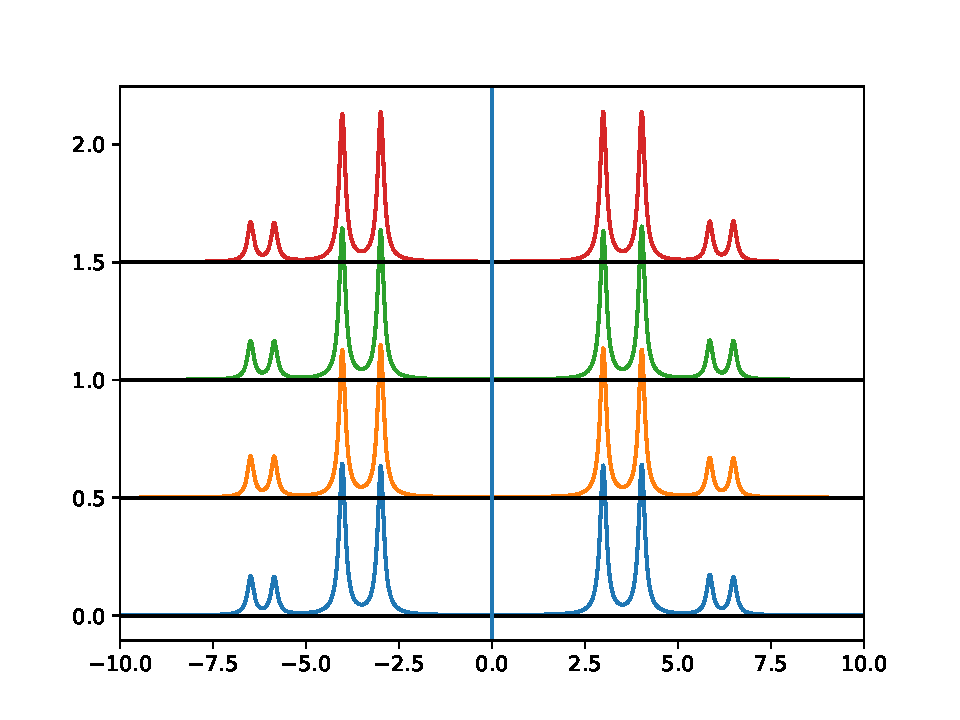
\includegraphics[width=0.95\textwidth]{figs/fig_tutorial.pdf}
                \end{center}
                \caption{Cette figure reproduit la figure de l'article
                \cite{peter}.}
                \label{fig:}
            \end{figure}


        % subsection Jeudi le 11 Mai (end)

    % section Semaine 2 (end)
\end{document}
